\documentclass[border=10pt]{standalone}
\usepackage[svgnames]{xcolor}
\usepackage{amsmath}
\usepackage{pgfplots}
\pgfplotsset{compat=newest}
\usepackage[sfdefault]{FiraSans}
\usepackage{FiraMono}
\renewcommand*\familydefault{\sfdefault}
\begin{document}
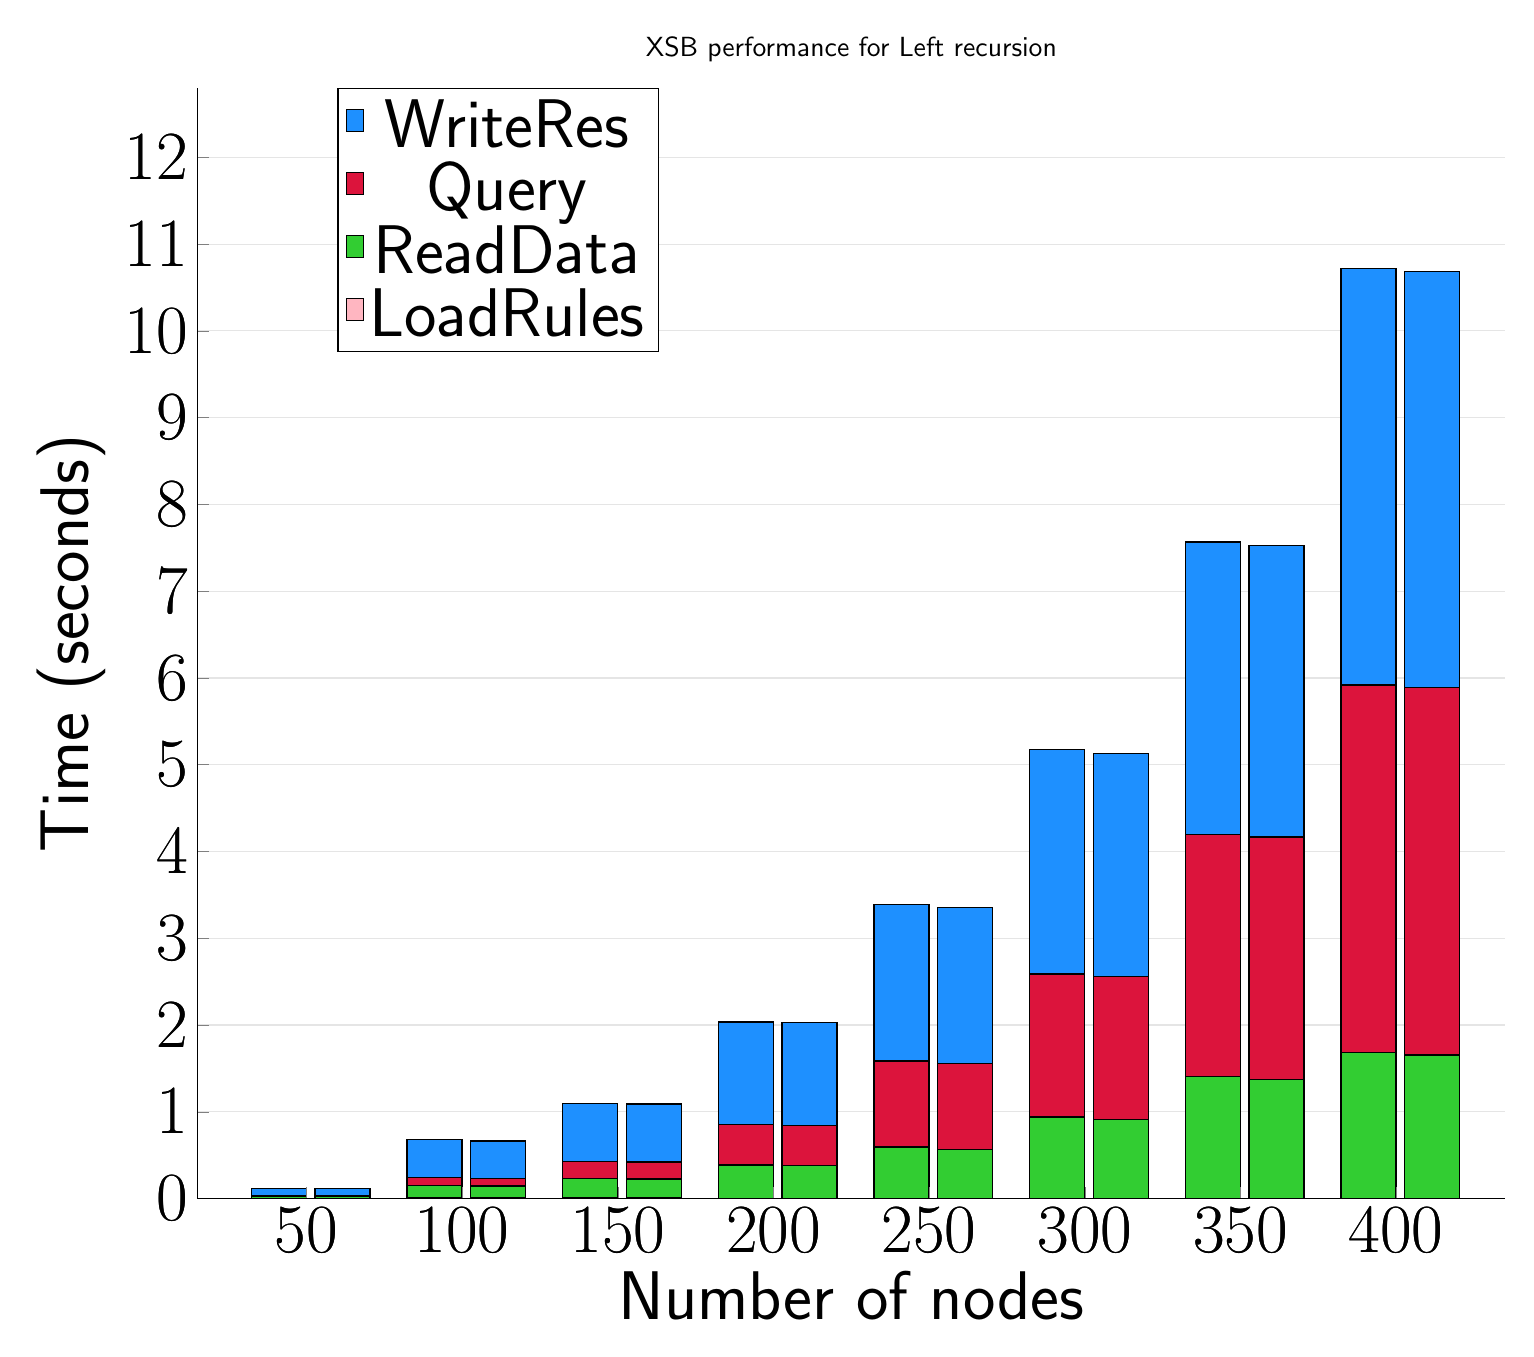
\begin{tikzpicture}
\begin{axis}[
   ybar stacked,
   title={XSB performance for Left recursion},
   bar shift=-10pt,
   width=1.5\textwidth,
   bar width=0.7cm,
   ymajorgrids, tick align=inside,
   major grid style={draw=gray!20},
   xtick=data,
   ymin=0, ymax=12.800821224848427,
   axis x line*=bottom,
   axis y line*=left,
   enlarge x limits=0.1,
   legend style={
       at={(0.23, 1)},
       anchor=north,
       legend columns=1,
       font=\Huge,
   },
   ylabel={Time (seconds)},
   xlabel={Number of nodes},
   label style={font=\Huge},
   tick label style={font=\Huge},
]
\addlegendimage{fill=DodgerBlue, draw=black, line width=0.2pt}
\addlegendentry{WriteRes}
\addlegendimage{fill=Crimson, draw=black, line width=0.2pt}
\addlegendentry{Query}
\addlegendimage{fill=LimeGreen, draw=black, line width=0.2pt}
\addlegendentry{ReadData}
\addlegendimage{fill=LightPink, draw=black, line width=0.2pt}
\addlegendentry{LoadRules}
\addplot +[fill=LightPink, draw=black, line width=0.5pt] coordinates {
    (50, 0.00356634457906087)
    (100, 0.004861911137898764)
    (150, 0.004883289337158203)
    (200, 0.0029783248901367166)
    (250, 0.0033263365427652967)
    (300, 0.0033350785573323534)
    (350, 0.00315999984741211)
    (400, 0.0030816396077473934)
};
\addplot +[fill=LimeGreen, draw=black, line width=0.5pt] coordinates {
    (50, 0.022935708363850903)
    (100, 0.148937702178955)
    (150, 0.22461835543314634)
    (200, 0.383572022120158)
    (250, 0.5899879932403567)
    (300, 0.936283270517985)
    (350, 1.4009226957956968)
    (400, 1.6804687182108566)
};
\addplot +[fill=Crimson, draw=black, line width=0.5pt] coordinates {
    (50, 0.007854302724202473)
    (100, 0.08602261543273933)
    (150, 0.19564199447631836)
    (200, 0.46464459101359035)
    (250, 0.992569367090861)
    (300, 1.6505170663197835)
    (350, 2.7949623266855834)
    (400, 4.236804405848186)
};
\addplot +[fill=DodgerBlue, draw=black, line width=0.5pt] coordinates {
    (50, 0.08455824851989746)
    (100, 0.4439271291097004)
    (150, 0.6723941167195636)
    (200, 1.1852313677469895)
    (250, 1.8023430506388325)
    (300, 2.5845168431599936)
    (350, 3.3667964140574167)
    (400, 4.800821224848427)
};
\end{axis}
\begin{axis}[
   ybar stacked,
   bar shift=13pt,
   width=1.5\textwidth,
   bar width=0.7cm,
   ymajorgrids, tick align=inside,
   major grid style={draw=none},
   xtick=data,
   ymin=0, ymax=12.800821224848427,
   axis x line*=none,
   axis y line*=none,
   enlarge x limits=0.1,
   label style={font=\Huge},
   tick label style={font=\Huge},
]
\addplot +[fill=LightPink, draw=black, line width=0.5pt] coordinates {
    (50, 0.003363)
    (100, 0.004844333333333333)
    (150, 0.004873333333333333)
    (200, 0.0024813333333333332)
    (250, 0.0028606666666666663)
    (300, 0.0033216666666666668)
    (350, 0.0028299999999999996)
    (400, 0.0022903333333333335)
};
\addplot +[fill=LimeGreen, draw=black, line width=0.5pt] coordinates {
    (50, 0.022923666666666665)
    (100, 0.13818866666666665)
    (150, 0.22122799999999998)
    (200, 0.38070266666666663)
    (250, 0.5642263333333334)
    (300, 0.9096676666666667)
    (350, 1.3678083333333335)
    (400, 1.6544413333333334)
};
\addplot +[fill=Crimson, draw=black, line width=0.5pt] coordinates {
    (50, 0.007850333333333334)
    (100, 0.085877)
    (150, 0.19569499999999998)
    (200, 0.46140566666666666)
    (250, 0.9926756666666666)
    (300, 1.6475333333333333)
    (350, 2.795145)
    (400, 4.230827000000001)
};
\addplot +[fill=DodgerBlue, draw=black, line width=0.5pt] coordinates {
    (50, 0.08429766666666667)
    (100, 0.43644066666666664)
    (150, 0.6691196666666667)
    (200, 1.1822226666666666)
    (250, 1.7963913333333335)
    (300, 2.571315333333333)
    (350, 3.364259)
    (400, 4.795075000000001)
};
\end{axis}
\end{tikzpicture}

\end{document}
